\subsubsection{الگوی \lr{Sanity Check}}
\label{archSafeSanityChkSec}
\begin{RTL}
این الگو \cite{ref4} در سیستم‌های نهفته بی‌درنگ یک روش سبک و کم‌هزینه
برای اطمینان از عملکرد معقول سیستم، حتی اگر کاملاً دقیق نباشد، است.
این الگو پوشش خطای حداقلی ارائه می‌دهد و برای شرایطی طراحی شده است که
کنترل دقیق برای ایمنی حیاتی نیست، اما اقدامات نادرست می‌توانند ضرر رسان باشند.
این الگو از حسگرهای ارزان‌قیمت و کم‌دقت برای شناسایی خطاهای قابل توجه
در عملکرد استفاده می‌کند و مطمئن می‌شود که سیستم در
صورت بروز انحرافات جزئی آسیب نمی‌بیند. این الگو یک نوع تغییر یافته از
\nameref{archSafeMonActSec} است که به یک حالت ایمن در صورت
بروز خطاهای بزرگ نیاز دارد و یک راه‌حل ساده و مقرون به صرفه
برای محافظت حداقلی فراهم می‌کند.
\end{RTL}
\begin{figure}[h!]
\centering
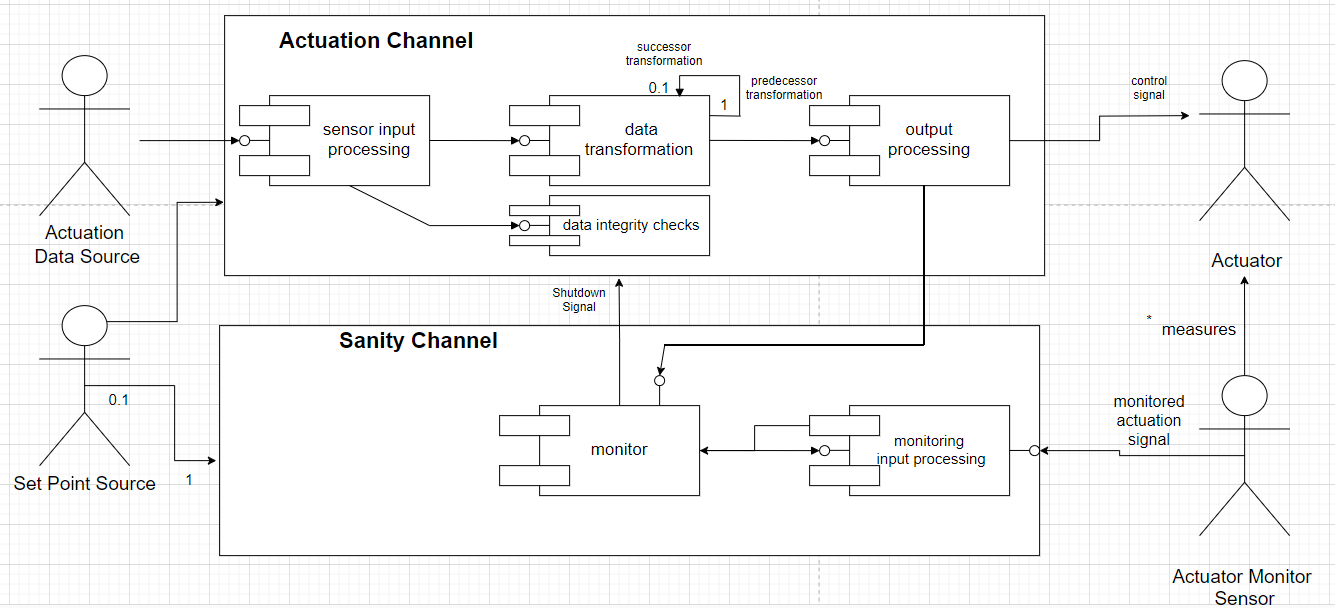
\includegraphics[scale=0.5]{images/third/sanityCheck.png}
\caption{ساختار الگوی \lr{Sanity Check}}
\end{figure}